\documentclass[12pt,oneside,a4paper,parskip]{scrbook}
\usepackage[utf8]{inputenc}
\usepackage{csquotes}
\usepackage[ngerman]{babel}
\usepackage{floatflt}
\usepackage{subfigure}
\usepackage[pdftex]{graphicx}
\usepackage[hidelinks]{hyperref}
\usepackage{color}
\usepackage{amssymb}
\usepackage{textcomp}
\usepackage{nicefrac}
\usepackage{scrhack}
\usepackage{pdfpages}
\usepackage{float}
\usepackage{pdflscape}
\usepackage{subfigure}
\usepackage{pdfpages}
\usepackage[verbose]{placeins}
%\usepackage[nouppercase,headsepline,plainfootsepline]{scrpage2}
\usepackage{listings}
\usepackage{xcolor}
\usepackage{color}
\usepackage{caption}
\usepackage{subfigure}
\usepackage{epstopdf}
\usepackage{longtable}
\usepackage{setspace}
\usepackage{booktabs}
\usepackage[style=numeric,backend=biber, uniquelist=false]{biblatex}
\bibliography{literatur}
\addbibresource{literatur.bib}


%%%%%%%%%%%%%%%%%%%
%% definitions
%%%%%%%%%%%%%%%%%%%
\def\BaAuthor{David Mödl\, Sebastian Lober}
\def\BaAuthorStudyProgram{Informatik} %% Wirtschaftsinformatik, E-Commerce, Informationssysteme
\def\BaType{Seminararbeit} %% Masterarbeit
\def\BaTitle{Bias of Neural Networks - Security implications}
\def\BaSupervisorOne{Prof.\ Dr.\ A B}
\def\BaSupervisorTwo{Prof.\ Dr.\ C D}
\def\BaDeadline{\today}

\ifdefined\iswithfullname
  \def\ShowBaAuthor{\BaAuthor}
\else
  \def\ShowBaAuthor{N.~N.}
\fi

\hypersetup{
pdfauthor={\ShowBaAuthor},
pdftitle={\BaTitle},
pdfsubject={Subject},
pdfkeywords={Keywords}
}

%%%%%%%%%%%%%%%%%%%
%% configs to include
%%%%%%%%%%%%%%%%%%%
\colorlet{punct}{red!60!black}
\definecolor{background}{HTML}{EEEEEE}
\definecolor{delim}{RGB}{20,105,176}
\colorlet{numb}{magenta!60!black}

\definecolor{gray}{rgb}{0.4,0.4,0.4}
\definecolor{darkblue}{rgb}{0.0,0.0,0.6}
\definecolor{cyan}{rgb}{0.0,0.6,0.6}

\definecolor{pblue}{rgb}{0.13,0.13,1}
\definecolor{pgreen}{rgb}{0,0.5,0}
\definecolor{pred}{rgb}{0.9,0,0}
\definecolor{pgrey}{rgb}{0.46,0.45,0.48}

\lstset{
  basicstyle=\ttfamily,
  columns=fullflexible,
  showstringspaces=false,
  commentstyle=\color{gray}\upshape
  linewidth=\textwidth
}

\lstdefinelanguage{json}{
    basicstyle=\normalfont\ttfamily,
    numbers=left,
    numberstyle=\scriptsize,
    stepnumber=1,
    numbersep=8pt,
    showstringspaces=false,
    breaklines=true,
    backgroundcolor=\color{background},
    literate=
     *{0}{{{\color{numb}0}}}{1}
      {1}{{{\color{numb}1}}}{1}
      {2}{{{\color{numb}2}}}{1}
      {3}{{{\color{numb}3}}}{1}
      {4}{{{\color{numb}4}}}{1}
      {5}{{{\color{numb}5}}}{1}
      {6}{{{\color{numb}6}}}{1}
      {7}{{{\color{numb}7}}}{1}
      {8}{{{\color{numb}8}}}{1}
      {9}{{{\color{numb}9}}}{1}
      {:}{{{\color{punct}{:}}}}{1}
      {,}{{{\color{punct}{,}}}}{1}
      {\{}{{{\color{delim}{\{}}}}{1}
      {\}}{{{\color{delim}{\}}}}}{1}
      {[}{{{\color{delim}{[}}}}{1}
      {]}{{{\color{delim}{]}}}}{1},
}

\lstset{language=xml,
  morestring=[b]",
  morestring=[s]{>}{<},
  morecomment=[s]{<?}{?>},
  stringstyle=\color{black},
  numbers=left,
  numberstyle=\scriptsize,
  stepnumber=1,
  numbersep=8pt,
  identifierstyle=\color{darkblue},
  keywordstyle=\color{cyan},
  backgroundcolor=\color{background},
  morekeywords={xmlns,version,type}% list your attributes here
}

\lstset{language=Java,
  showspaces=false,
  showtabs=false,
  tabsize=4,
  breaklines=true,
  keepspaces=true,
  numbers=left,
  numberstyle=\scriptsize,
  stepnumber=1,
  numbersep=8pt,
  showstringspaces=false,
  breakatwhitespace=true,
  commentstyle=\color{pgreen},
  keywordstyle=\color{pblue},
  stringstyle=\color{pred},
  basicstyle=\ttfamily,
  backgroundcolor=\color{background},
%  moredelim=[il][\textcolor{pgrey}]{$$},
%  moredelim=[is][\textcolor{pgrey}]{\%\%}{\%\%}
}

\newcommand*{\forcetwosidetitle}[1][1]{%
 \begingroup
   \cleardoubleoddpage
   \KOMAoptions{titlepage=true}% useful e.g. for scrartcl
   \csname @twosidetrue\endcsname
   \maketitle[{#1}]
 \endgroup
}


\begin{document}


%%%%%%%%%%%%%%%%%%%
%% Titelseite
%%%%%%%%%%%%%%%%%%%


\frontmatter
\titlehead{%  {\centering Seitenkopf}
  {Hochschule für angewandte Wissenschaften Würzburg-Schweinfurt\\
   Fakultät Informatik und Wirtschaftsinformatik}}
\subject{\BaType}
\title{\BaTitle\\[15mm]}
%\subtitle{\normalsize{vorgelegt an der Hochschule f\"{u}r angewandte Wissenschaften W\"{u}rzburg-Schweinfurt in der Fakult\"{a}t Informatik und Wirtschaftsinformatik zum Abschluss eines Studiums im Studiengang \BaAuthorStudyProgram}}
\author{David Mödl \& Sebastian Lober}
%\date{\normalsize{Eingereicht am: \BaDeadline}}
%\publishers{
%  \normalsize{Erstpr\"{u}fer: \BaSupervisorOne}\\
%  \normalsize{Zweitpr\"{u}fer: \BaSupervisorTwo}\\
%}
\forcetwosidetitle


%%%%%%%%%%%%%%%%%%%
%% abstract
%%%%%%%%%%%%%%%%%%%

\section*{Zusammenfassung}

TODO

\section*{Abstract}
KI steht kurz für künstliche Intelligenz. Der Begriff KI ist jedoch irreführend. Eine 'KI' ist ein Programm, das versucht biologisches intelligentes Verhalten nachzuahmen. Die Begrifflichkeit Intelligenz in Verbindung mit Computern ist sehr umstritten, dennoch wird im Allgemeinen als auch in der Forschung das Wort 'Intelligenz' verwendet. \\
Aus diesem Grund und an Mangel an qualitativ hochwertigen Alternativen wird auch im Folgenden der Wortlaut KI verwendet, wohl wissend, dass die Bezeichnung nicht 100 Prozent korrekt ist.

%%%%%%%%%%%%%%%%%%%
%% Inhaltsverzeichnis
%%%%%%%%%%%%%%%%%%%
\tableofcontents



%%%%%%%%%%%%%%%%%%%
%% Main part of the thesis
%%%%%%%%%%%%%%%%%%%
\mainmatter

\chapter{Einführung}
\label{chapter:intro}
Künstliche Intelligenz(KI) oder auch artifizielle Intelligenz(AI) tritt allgegenwärtig in großen Teilen unserer Gesellschaft auf. Von Kaufvorschlägen auf Amazon, über Chat-Bots bis hin zu autonom fahrenden Autos spielt die KI eine große Rolle. Ein bekanntes Beispiel ist die Software "alpha go", welche den internationalen GO Champion Lee Sedol besiegte\cite{alphaGo}. Darüber hinaus ermöglicht die KI komplexe Sachverhalte zu simulieren und zu prognostizieren, wie zum Beispiel die vollautomatische Generierung hochaufgelöster, realistischer Videosequenzen auf der Grundlage simpler Eingaben\cite{videoToVideo}.
\\\\
Einerseits gibt es viele Erfolge, die für ein KI betriebenes System sprechen. Andererseits bestärken medienwirksame Verfehlungen, wie z.B. das frauenfeindliche Bewerbungssystem von Amazon\cite{amazon}, die Skeptiker solcher Systeme. Ziel dieser Arbeit ist es, die unterschiedlichen Ursprünge solcher algorithmischen Verzerrungen (engl. bias) zu erläutern und Präventionen zu schildern, welche diese vermeiden sollen.
\\\\
Wir beginnen unsere Arbeit damit, Grundlagen für ein fundamentales Wissen spätere Kapitel aufzubauen. Danach möchten wir auf die Entstehung solcher Bias eingehen, die damit verbundenen Probleme und welche Präventionen gegen diese Fehlverhalten unternommen werden können.
\chapter{Grundlagen}
\section{Bias}
Wesentlicher Bestandteil der Arbeit ist das erläutern der "Biases", welche durch die Nutzung von künstlicher Intelligenz auftreten können. Das Wort Bias kommt aus dem Englischen und bedeutet im Wesentlichen:

\begin{enumerate}
	\item Verzerrung – im statistischen Sinn als mittlere systematische Abweichung zwischen dem erwarteten („richtigen“) Modellergebnis und dem mittleren wirklich eingetretenen Modellergebnis.
	\item Voreingenommenheit – je nachdem, wie wir die Welt aufgrund unserer Erfahrungen sehen, kommen wir zu unterschiedlichen Schlüssen.
\end{enumerate}

Der Begriff Voreingenommenheit muss bei der Nutzung von KI vorsichtig behandelt werden, denn eine Maschine besitzt grundsätzlich keinerlei Vorurteile und weiß zu Beginn nicht was richtig oder falsch ist. Hier spricht man daher von einem Fehlverhalten oder einer Verzerrung, welche durch äußere Einflüsse wie z.B. dem Menschen verursacht wurden.\\

\section{Künstliche Intelligenz}
Künstliche Intelligenz (KI) oder englisch artificial intelligence (AI) ist der Oberbegriff für ein Teilgebiet der Informatik. Dieses Gebiet befasst sich nicht nur mit neuronalen Netzen, sondern generell mit jeglicher Form von maschinellen intelligenten Verhalten und dem maschinellen Lernen, siehe Abbildung \ref{fig:Uebersicht}. Generell wird bei der künstlichen Intelligenz versucht biologische Intelligenz auf einen Computer zu simulieren. Dies basiert meist auf simplen Algorithmen, wodurch die Begrifflichkeit 'Intelligenz' in Bezug auf einer Maschine öfter in Frage gestellt wird.
% Oder hier irgenwas zitieren hier.
% Das Rad muss nicht immer neu erfunden werden.

\begin{figure}[ht]
	\begin{center}
		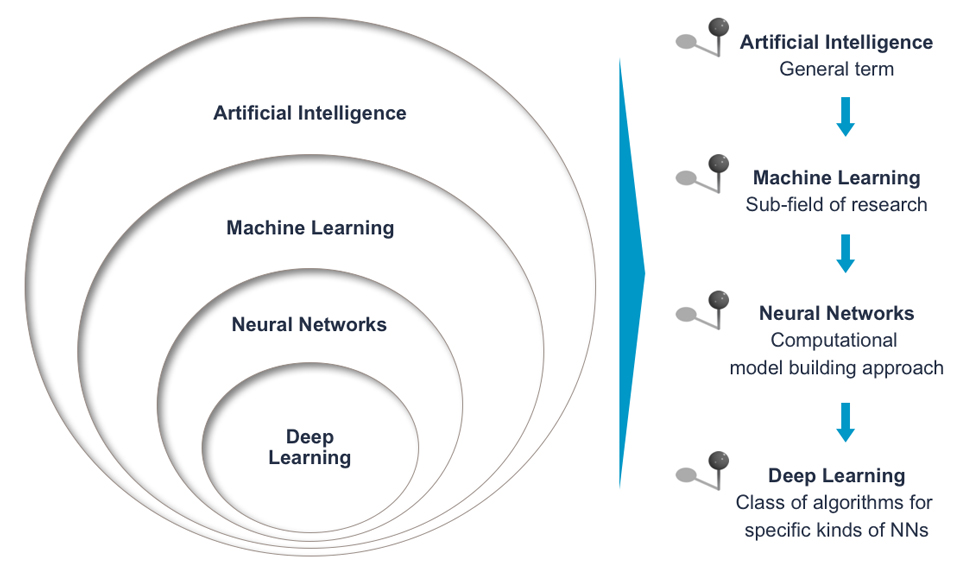
\includegraphics[width=14cm]{Bilder/Abstraktionslevel_von_AI.jpg}
		\caption{Verschiedene Abstraktionslevel von Artificial Intelligence in hierarchischer Ordnung}
		\label{fig:Uebersicht}
	\end{center}
\end{figure}
%https://www.capgemini.com/de-de/2017/09/artifical-intelligence-machine-learning-und-data-science-same-same-but-different/
Damit ein Programm den Titel KI tragen darf, muss sie zum einen die Fähigkeit zu lernen besitzen, zum anderen die Fähigkeit intelligent Lösungen zu finden, auch bei nicht eindeutigen Eingaben.\\
KIs werden grob in zwei Kategorien aufgeteilt. Einmal die starke KI, die ebenbürtig mit Menschen zusammenarbeiten kann und schwacher KI, die lediglich das Arbeiten von Menschen unterstützen soll.
% symbolische vs. neuronale KI
% Simulationsmethode vs. phänomenologische Methode
% Problemlösungsansätze: Suchen, Planen, Optimieren, logisches Schließen, Approximieren
\subsection{Maschine Learning}
Machine Learning (ML) ist ein Teilgebiet der künstlichen Intelligenz. Es ist der Oberbegriff jeglicher Lernvarianten von KIs. Im Allgemeinen versucht eine KI neue Muster und Gesetzmäßigkeiten in Trainingsdaten zu erkennen, diese zu verallgemeinern und für neue Problemlösungen oder für die Analyse von bisher unbekannten Daten zu verwenden\cite{EliminateHumanBias}.
\\\\Diese Arbeit speziell konzentriert sich auf Deep Learning, welches eine Variante zum Trainieren von neuronalen Netzen darstellt.
\subsubsection{Lernansätze}
KIs bestehen aus vielen Algorithmen. Damit eine KI lernt, müssen diese Algorithmen angepasst werden. Dies kann überwacht geschehen mittels eines "Lehrers", der den Lernerfolg bei evolutionären Algorithmen-Änderungen überprüft.\\
Die andere Variante ist das unüberwachte Lernen. Hierbei erzeugt ein Algorithmus ein statisches Model aus den Trainingsdaten und erkennt Zusammenhänge zwischen den Daten und dessen Kategorie, sogenannte Features. Diese System gibt die Wahrscheinlichkeit zurück, zu welcher Kategorie die Eingabe gehört, abhängig von den erkannten Features der Eingabe.\\\\
Aus den Konzept dieser zwei Hauptlernvarianten wurden diverse Unterlernvarianten erstellt, wie teilüberwachtes Lernen, bestärktes Lernen oder unüberwachten Lernen ohne Kategorisierung.
\subsection{Neuronale Netze}
Künstliche neuronale Netze (KNN) bestehen aus künstlichen Neuronen, die untereinander verflechtet sind. Diese Konstrukte sind denen der Neuronen-Verbindungen im Nervensystem eines Lebewesens nachempfunden. \\
KNNs sind nicht dazu da das Nervensystem von Lebewesen nachzubilden, sondern abstrakt die Eigenschaften der Informationsverarbeitung und der Lernfähigkeit zu imitieren.

\begin{figure}[h]
	\begin{center}
		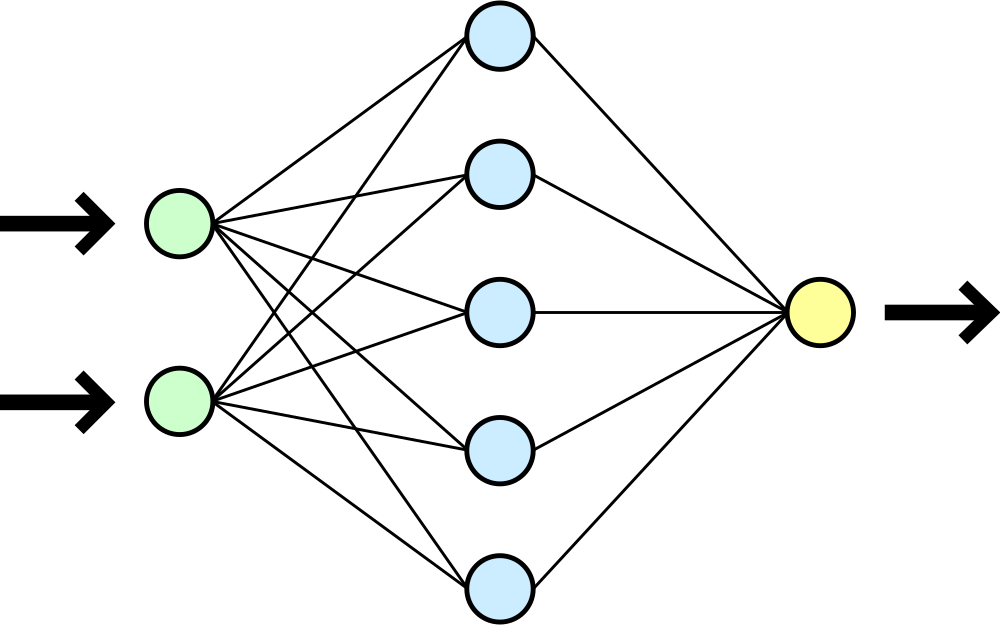
\includegraphics[width=12cm]{Bilder/Neurales_Netz.png}
		\caption{Vereinfachte Darstellung eines künstlichen neuronalen Netzes}
		\label{fig:wikiNeuronalesNetz}
	\end{center}
\end{figure}
% https://de.wikipedia.org/wiki/K%C3%BCnstliches_Neuron#/media/Datei:ArtificialNeuronModel_deutsch.png

KNNs sind meist in Schichten mit beliebig vielen künstlichen Neuronen aufgebaut. In der Regel besteht ein KNN aus drei Teilen die Eingangsschicht (grün), verdeckte Schicht (blau) im Englischen Hidden Layer und die Ausgabeschicht (gelb). In der Eingangsschicht fließen die Informationen in das Netz ein und in der Ausgabeschicht das Ergebnis der Berechnungen aus. Jede Schicht besteht aus beliebig vielen Neuronen je nach Komplexität des Zieles, die Hidden Layer sogar aus beliebig viele Schichten.
\\\\
In der Regel arbeiten KNNs nach dem feedforward-Prinzip, bei dem die Informationen immer nur in eine Richtung fließt. Es gibt jedoch auch rekurrente Netze, bei denen durch rückgerichtete Kanten Rückkopplungen im Netz entstehen. \\
Die einfachste Netzstruktur ist das einschichtige feedforward-Netz. Dies besteht ohne Rückkopplungen aus nur einer Schicht, der Ausgabeschicht.
\subsubsection{Das künstliche Neuron}
Künstliche Neuronen sind die Grundbestandteile eines künstlichen neuronalen Netzes.
Ein künstliches Neuron ist die vereinfachte und abstrakte Version einer biologischen Nervenzelle und ist wie folgt aufgebaut.\\
\begin{figure}[h]
	\begin{center}
		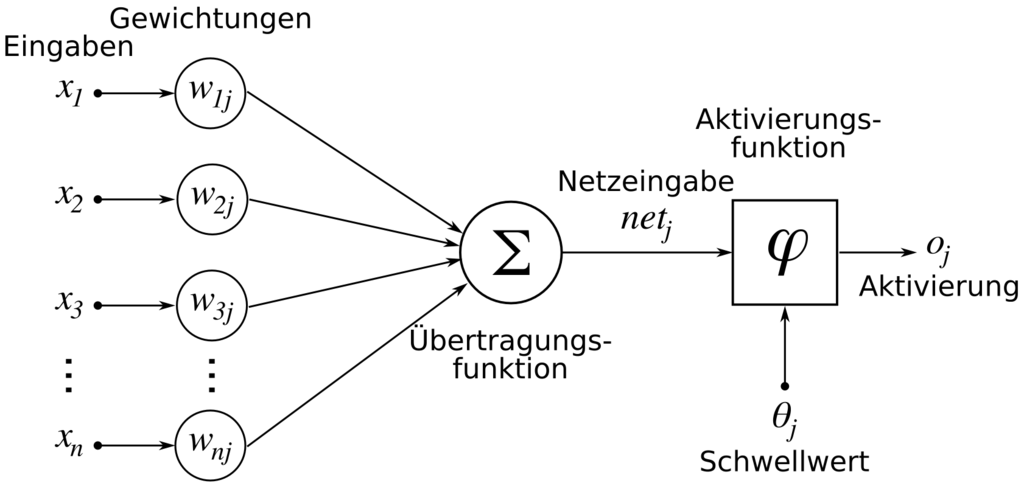
\includegraphics[width=12cm]{Bilder/ArtificialNeuronModel_deutsch.png}
		\caption{Ein künstliches Neuron}
		\label{fig:wikiNeuron}
	\end{center}
\end{figure}
% https://de.wikipedia.org/wiki/K%C3%BCnstliches_Neuron#/media/Datei:ArtificialNeuronModel_deutsch.png

Ein künstliches Neuron besitzt $n$ Eingangskanäle und einen Ausgangskanal. $j$ repräsentiert hier die eindeutige Nummer des Neuron. Jede Eingabe $x_{i}$ besitzt ein dazugehörendes Gewicht $w_{1j}..w_{nj}$. Dieser spiegelt die Wichtigkeit der Eingabe wider, diese kann hemmend negativer oder erregend positiver Wert wirken. Die Übertragungsfunktion $\Sigma$ summiert alle multiplizierten Eingaben mit ihrem Gewicht und geht als Netzeingabe $net_j$ in die Aktivierungsfunktion $\varphi$ ein. \\
Ob das Neuron "'feuert"' oder kein Signal sendet, wird hier berechnet. Auf die Netzeingabe $net_j$ wird ein Schwellenwert $\theta_j$ addiert. Als mathematisch Vereinfachung wird der Schwellwert $\theta$ als $w_0$ bezeichnet und $x_0 = 1$ eingeführt und somit in der folgenden Formel immer auf die Netzeingabe $net_j$ addiert.
\\\\
${\displaystyle a=\sum _{i=0}^{n}x_{i}w_{i}}$
\\\\
Die Variabel $a$ geht in die Aktivierungsfunktion ${\sigma (a)}$ ein, anhängig von dem Ergebnis wird das Neuron aktiv oder bleibt inaktiv.
Der Ausgangskanal eines Neuron ist gleichzeitig ein Eingangskanal eines oder mehreren anderen Neuronen.
\\\\
Dadurch dass ein Neuron mehrere Eingangskanäle besitzt, werden viele Eingangsinformationen auf ein Ergebnis reduziert. Durch mehrere Schichten und vielen Neuronen pro Schicht kann so eine große Menge an Daten schnell reduziert werden.
\\\\
Jedoch muss jedes künstliche Neuron eines KNNs richtig eingestellt werden, damit das KNN dessen Ziel erfüllt. Eingestellt wird das Neuron durch Training. Trainieren bedeutet hier das Ermitteln der richtigen Werte für Gewichtungen und Schwellwerte, als auch das Einstellen der richtige Verbindungskombinationen der Neuronen untereinander. Diesen Prozess nennt man Deep Learning, eine Form von Machine Learning.
\subsection{Deep Learning}
Deep Learning ist eine Maschine Learning Variante, die speziell bei künstliche neuronale Netze eingesetzt wird. Beim Deep Learning werden die zahlreichen Zwischenschichten der Hidden Layer trainiert. Dabei wird eine umfangreiche und komplexe Struktur der Neuronen-Verbindungen aufgebaut. Wie das Programm endgültig die Aufgabe lösen soll, wird hierbei nicht vorgegeben, sondern wird bei diesem autonomen Prozess evolutionär ermittelt.
%\begin{figure}[h]
%	\begin{center}
%		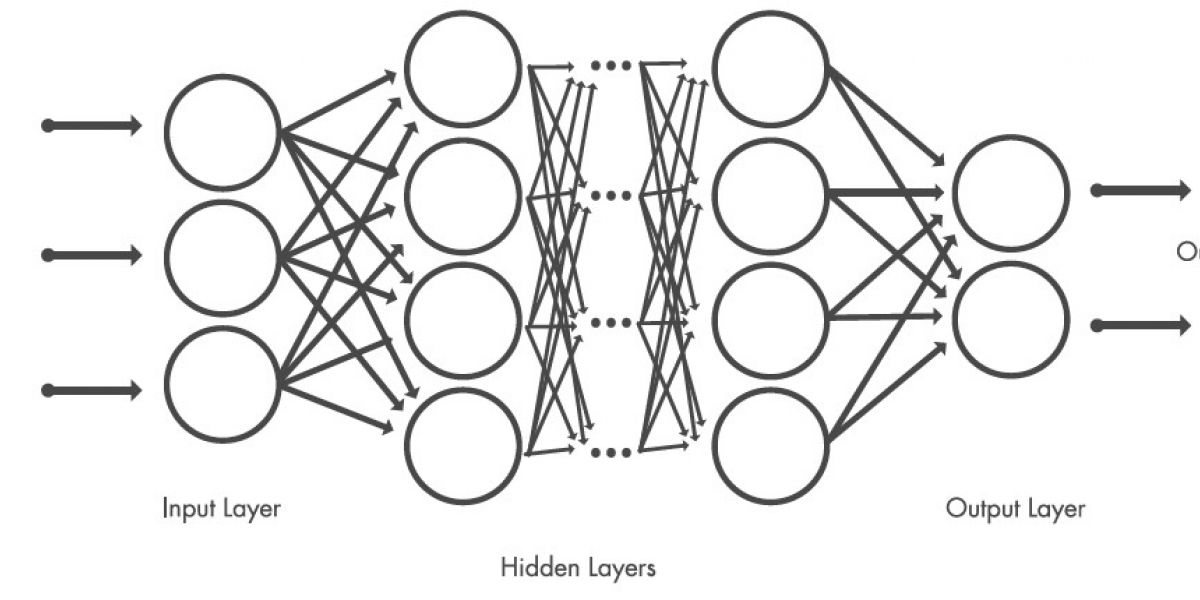
\includegraphics[width=15cm]{Bilder/Deep-Learning.jpg}
%		\caption{Hidden Layer}
%		\label{Deep Learing von Technik-und-Wissen}
%	\end{center}
%\end{figure}
% https://www.technik-und-wissen.ch/assets/images/4/1-Mathworks-Deep-Learning-80166094.jpg
\\\\
Ein künstliches neuronales Netz wird mit dem Zweck aufgebaut, eine bestimmte Aufgabe zu lösen. Extra dafür müssen Trainingsdaten aufbereitet werden. Diese Art der Daten, beispielsweise Bilder, soll das fertig trainierte Netz richtig interpretieren können. Trainings und Testdaten sind Daten, bei dem das korrekte Ergebnis bekannt ist.
\\\\
Am Anfang ist das künstliche neuronale Netz meist mit relativ zufälligen Werten und Verbindungen vorbelegt. Trainingsdaten werden dem zu trainierenden Netzwerk an die Eingangsschicht übergeben. Diese durchlaufen das Netz. Das Ergebnis wird an der Ausgabeschicht überprüft. Die Ausgabeschicht besteht im einfachsten Fall aus zwei Neuronen, beispielsweise "'Gesicht erkannt"' oder "'kein Gesicht"', an dem gemessen wird, wie viel gewichtete Signale ankommen. Diese summiert, ergeben die Endergebnisse der Berechnungen und das Neuron mit dem höchsten Gewicht, ergibt die Antwort.
\\\\
Neuronale Netze sind für Menschen ab einer gewissen Größe nicht mehr nachvollziehbar. Somit kann nur die Eingabe mit der Ausgabe mit Hilfe von Testdaten verglichen werden, um auf die Korrektheit der Aufgabenlösung zu prüfen. Ziel ist es mit möglichst vollständigen Trainingsdaten das Netzwerk so einzustellen, dass diese nicht nur die Trainingsdaten und Testdaten richtig beantwortet, sondern auch unbekannt Daten korrekt interpretiert.
\\\\
Um eine Aufgabe, wie 'Gesicht in Bild erkennen', zu trainieren, wird nicht nur ein Netz mit Zufallswerten und Verbindungen generiert sondern tausende. Alle werden mit den gleichen Testdaten geprüft und für jedes Netz ein Mittelwert über die Korrektheit der Antworten erstellt. Da alle Netze Initial mit Zufallswerten belegt sind, haben die meisten Netze eine Erfolgsrate von ca. 50 Prozent. Die Netze mit den höchsten Erfolgsraten, mit beispielsweise mehr als 60 Prozent, werden behalten, der Rest wird verworfen. Die erfolgreichsten Netze werden mehrfach kopiert und bei jedem Kopiervorgang individuell leicht verändert und erneut getestet. Die Besten werden wieder genommen und leicht modifiziert kopiert und schlechteren verworfen.
\\\\
Nach einer gewissen Anzahl an Iterationen entscheidet das Netz nicht mehr willkürlich, sondern scheint intelligent die Aufgabe zu lösen. Dieser Iterationsschritt kann unendlich oft laufen, jedoch empfiehl es sich, je nach Anwendungsfall, ab einer gewissen Erfolgsrate das Training zu beenden oder neue Trainings- und Testdaten zu verwenden. Als Ergebnis des Prozesses erhält man durch Deep Learning ein trainiertes künstliches neuronales Netz, das im Allgemeinen als KI bezeichnet wird.

\subsection{Loss-Funktion}
\label{section:lossFunction}

Alle Modelle benötigen eine Loss-Funktion(Verlustfunktion), um später trainiert werden zu können. Die Verlustfunktion bestimmt die Differenz zwischen der Prognose, die das Modell liefert, und dem vorgegebenen Label. Sie muss für die Menge aller Daten berechnet werden und beschreibt damit, wie gut das Modell die Trainingsdaten abbildet. 
% Schreiben
%https://www.ai-united.de/arbeitsweise-eines-neuronalen-netzwerkes-algorithmen-training-aktivierungs-und-verlustfunktionen/
%https://www.sigs-datacom.de/trendletter/2018-06/12-werkzeugneutrale-einfuehrung-in-maschinelles-lernen.html
\subsection{Informationsverlust zwischen Schichten}
1.	Erste Schicht verbunden mit letzter Schicht\\
	a.	Eingabe hoher Einfluss auf Endergebnis\\
2.	Jede Schicht nur Verbindung zu der Nächsten\\
	a.	Hohe Informationsverlust\\

\section{Architekturen}
Arten
\\1.	Full Connected
\\2.	CNN
\\3.	ResNet
\\4.	Natural Network Connection
\\5.	Dropout
\\6.	…

\section{Daten}
\label{section:Data}
Erst durch eine Kombination aus Algorithmen und Daten wird die Entscheidungsfindung unterstützt. Wie ein menschlicher Entscheider können auch Algorithmen wegen unvollständiger oder fehlerhafter Daten zu fehlerhaften Entscheidungen gelangen.
Deswegen sollte bei der Datenaufbereitung bereits darauf geachtet werden die richtige Woge zwischen Quantität und Qualität zu finden.

\subsection{Quantität}
\label{section:DataQuantity}
Je breiter, also je mehr Variablen in den Datensätzen existieren, umso komplexer wird die Aufgabe. Und diese Komplexität der Probleme erfordert, dass die Menge an Daten entsprechend groß sein muss, damit das zu trainierende System immer besser reagiert.
\\\\
Ein Beispiel hierfür findet sich in der Autoindustrie. Beim autonomen Fahren müssen Daten von Laser-, Kamera- und Radarsensoren im Auto zuverlässig und schnell verarbeitet und zusammengeführt werden. Dadurch verfügt das Fahrzeug jederzeit über ein präzises Abbild der realen Verkehrsbedingungen, kann sich selbst in diesem Umfeld verorten und darauf basierend in jeder Fahrsituation die richtige Entscheidung treffen \cite{autonomesFahren}.
\\\\
Anhand dieses Beispiels erkennt man die Wichtigkeit der Quantität der Trainingsdaten, da die Anzahl möglicher Situationen im Straßenverkehr prinzipiell unendlich ist. Um gleichartige Strukturen im Verkehrsgeschehen zu erkennen, sind viele Trainingsdaten erforderlich, die ein immer genaueres Bild ergeben.
\\\\
Da aber nicht immer die Anwendungen komplex sind, sind nicht immer viele Datensätze notwendig. Bei geringerer Komplexität reichen somit weniger Datensätze aus um gute Ergebnisse zu erreichen.

\subsection{Qualität}
\label{section:DataQuality}
Auch die Qualität der Trainingsdaten spielt eine wichtige Rolle. Die Datenqualität zeichnet sich dadurch aus, dass Daten den Zweck in einem bestimmten Zusammenhang erfüllen müssen. 
\\\\
Dass heißt wenn nun die KI auf Bildern z.B. einen Panzer erkennen soll\cite{panzer}, muss die KI mit Bildern von Panzern trainiert werden, welche auch als Panzer gekennzeichnet wurden.
Würden nun Bilder von Autos mit in die Testdaten gelangen, welche auch zuvor als Panzer gekennzeichnet wurden, würde die Maschine diese Autos bei unbekannten Bildern auch als Panzer erkennen.
\\\\
Daher ist es für den Erfolg der Daten die Qualität dieser sehr wichtig. Hierbei sollten somit keine unzweideutigen Stammdaten existieren.

%% Vollständigkeit erwähnen, z.B. auch andere Kulturen beachten usw.
%% Panzer problem in Unvollständigkeit der Daten aufgreifen. Und sagen, dass natürlich die Qualität nicht so stimmen muss, sondern auch solche Fälle abdeckt, dass ein Panzer bei unterschiedlichsten Wetter gefahren werden kann.

\chapter{Bias Entstehung}
Bei der Nutzung von KI System können Verzerrungen(Bias) bzw. Fehlverhalten entstehen, diese können unterschiedlicher Natur sein und an unterschiedlichen Stellen, in der in Abbildung \ref{fig:dataBias} gezeigten, vereinfachten Machine Learning Pipeline, auftreten. Dabei möchten wir auf die Daten eingehen, welche bei der Eingabe zu Bias führen können und menschliche Fehler verdeutlichen, welche bei der Verarbeitung und der Ausgabe auftreten können. Zuletzt möchten wir Adversial Attacks ansprechen, welche zu weiteren Verzerrungen führen können.

\begin{figure}[h]
	\begin{center}
		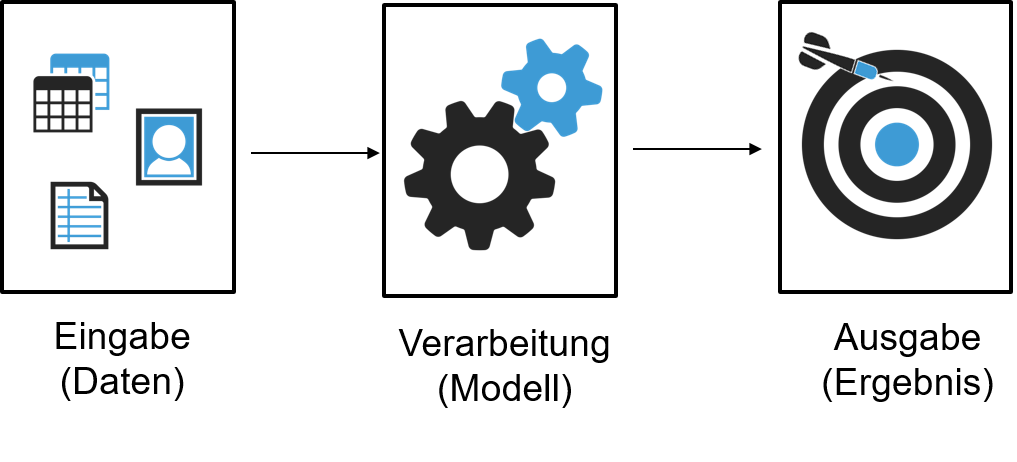
\includegraphics[width=12cm]{Bilder/data_bias.png}
		\caption{Machine Learning Pipeline: Eingabe, Verarbeitung, Ausgabe}
		\label{fig:dataBias}
	\end{center}
\end{figure}

\section{Daten}
\label{section:data}
Im ersten Kapitel möchten wir erläutern welche Bias, durch z.B. eine schlechte Datenqualität oder Datenquantität, entstehen können.

\subsection{Unvollständigkeit der Daten}
\label{section:uncompleteData}
Zuerst möchten wir auf ein Problem aufmerksam machen, welches zu Verzerrungen führt, anhand des Beispiels aus \ref{section:DataQuality}.
\\\\
Das Pentagon hatte eine Software angefordert, welche Panzer in der Natur erkennen sollte. KI Forscher haben daraufhin ihr neuronales Netz mit Fotos von getarnten Panzern trainiert, und mit Landschaftsfotos ohne getarnte Panzer. Dadurch sollte gewährleistet werden, dass die Software Panzer auf unbekannten Bildern erkennt.
\\\\
Bei internen Test funktionierte das System sehr gut, doch bei den realen Test schien die Software nicht zu funktionieren. Das Problem hierbei lag daran, dass diese KI zuvor mit Trainingsdaten gefüttert wurde, welche nur bei schönem Wetter fotografiert wurden (siehe \hyperref{fig:tank}). Auch die internen Testdateien erfüllten dieses Kriterium. Die realen Test hingegen wurden bei jedem Wetter ausgetragen.

\begin{figure}[h]
	\begin{center}
		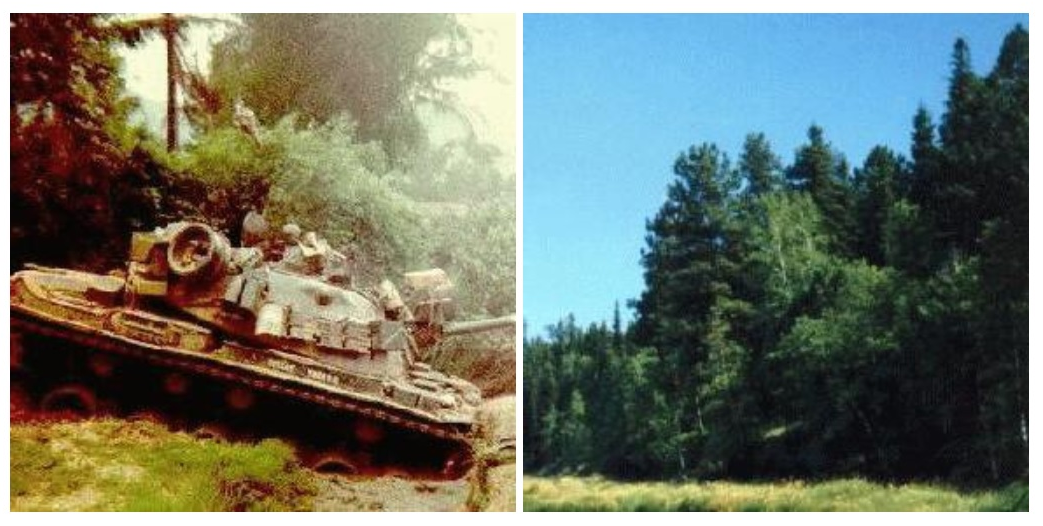
\includegraphics[width=15cm]{Bilder/tank.png}
		\caption{Panzer bei bewölkten Wetter vs Landschaft ohne Panzer bei schönem Wetter}
		\label{fig:tank}
	\end{center}
\end{figure}
Die Software hatte somit trainiert schlechtes und gutes Wetter auseinander zu halten und nicht Panzer zu erkennen. Das Problem hierbei lag an unvollständigen Daten, hier wurden zu wenig unterschiedliche Fälle getestet und dadurch wurde ein Bias erzeugt, welcher die Nutzung der Software unmöglich machte.

\subsection{Garbage in - Garbage out}
\label{section:DataGarbage}
Eine Maschine kennt grundsätzlich keinen Unterschied zwischen Schwarz und Weiß, Mann und Frau oder Jung und Alt. Erst durch eine KI lernt eine Maschine Verhalten und Muster kennen. Hierfür werden wie bereits in \ref{section:Data} beschrieben Daten benötigt, welche die richtige Qualität benötigen um die Ergebnisse zu bestimmen.
\\\\
Bleiben fehlerhafte Daten unentdeckt, wird ein System trainiert, welches in Zukunft falsche Ergebnisse liefern wird. Das Beispiel aus \ref{section:DataQuality} erläutert dieses Problem. Möchte ich ein System trainieren, welches Panzer identifizieren kann, muss ich diesem System beibringen Panzer zu erkennen. Füttere ich dieses nun mit Autos und markiere diese versehentlich als Panzer, identifiziert das System daraufhin diese nicht als Autos sondern als Panzer.
\\\\
Bei der traditionellen  Datenanalyse können solche schlechte Daten nachträglich entfernt werden. Hat allerdings eine Maschine durch maschinelles Lernen etwas gelernt, wird es schwer dies wieder zu verlernen. Denn ab einem Gewissen Grad wird es nahezu unmöglich, herauszufinden, auf welche Datenelemente die Vorhersagen basieren. Ähnlich wie beim menschlichen Gehirn.\\
Baut unser erlerntes Wissen in Teilen auf falsche Grundannahmen oder Informationsbausteinen auf, verliert der ganze Komplex seinen Wert und wir müssen von neu alles erlernen.
\\\\
Diese Problem wird in der KI als "Garbage in - Garbage out" (Müll rein, Müll raus) bezeichnet.

\subsection{Bias in Trainings-/Testdaten}
\label{section:biasInTest}
Ca. 4 Jahre entwickelte Amazon einen Algorithmus, welcher unter mehreren Bewerbungstexten automatisch die besten Bewerber herausfiltern sollte. Dabei bezog die Software sich auf voran gegangene Bewerbungen, verdeutlichte dabei aber ein grundlegendes Problem des maschinellen Lernens in seiner aktuellen Form.\\\\
Der Algorithmus hatte mit den Datensätzen der angenommen Bewerber trainiert und lernte daraus welche Eigenschaften Amazon bevorzugt. Weil das Unternehmen aber Teil einer von Männern dominierten Industrie ist, waren in den zugrunde gelegten vergangenen zehn Jahren vor allem Männer eingestellt worden. Daraus resultierte, dass Frauen grundsätzlich schlechter bewertet wurden, selbst ohne die Angabe eines Geschlechtes und dieses z.B. nur durch Frauenvereine erkennbar wurde. Die KI blieb diesen Auswahlkriterien treu und bevorzugte vorwiegend Männer.\cite{amazon}
\\\\
Die Hoffnung solcher Anwendungen liegt eigentlich darin, Vorurteile zu vermeiden und Prozesse fairer zu gestalten, da eine Maschine wie in \ref{section:DataGarbage} bereits genannt keine Unterschiede kennt. Doch in diesem Beispiel beinhalteten die Trainingsdaten bereits Vorurteile und führten somit zu einem Fehlverhalten des Systems.
\\\\
%Beispiel von Tay The Chatbot zeigen, für Beispiel Bias in Testdaten?
An diesem Beispiel wird deutlich wie zentral die Daten für eine KI sind.
Meist ist es nicht möglich Daten zu finden, welche nicht bereits menschliche Bias enthalten. Solch verzerrte Trainingsdaten, werden unter Bezug auf ihre Zusammensetzung auch als WEIRD Samples (western, educated, industrialized, rich and democratic societies) bezeichnet\cite{BiasInKi}.


\subsection{Under-/ Overfitting}
\label{section:OverUnderfitting}

Wie in \ref{section:DataQuantity} bereits beschrieben, spielt die Datenquantität eine große Rolle beim maschinellen Lernen. Die beiden Fehler die allerdings dadurch entstehen können, sind nutzloses Wissen aufzubauen oder aus einem vorhandenem Trainingsdatensatz keine Relevanten Lerninformationen ziehen zu können. Diese Phänomene werden als Overfitting (Überanpassung) und Underfitting(Unteranpassung) bezeichnet.

\begin{figure}[h]
	\begin{center}
		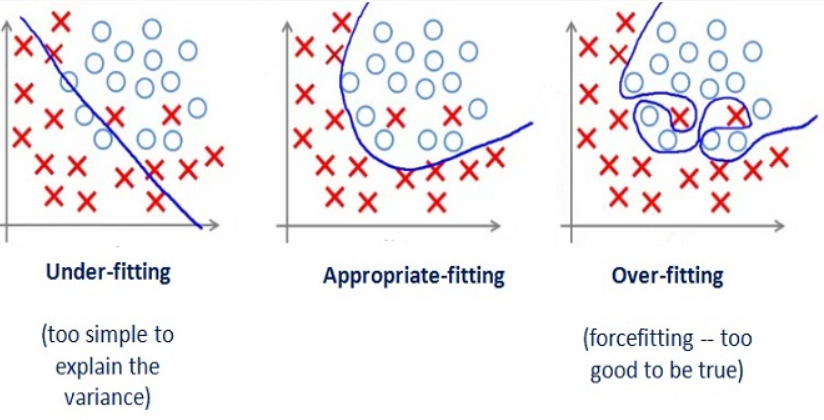
\includegraphics[width=15cm]{Bilder/overUnderfitting.png}
		\caption{Over- und Underfitting}
		\label{fig:overUnderFitting}
	\end{center}
\end{figure}

Der linke Graph aus \ref{fig:overUnderFitting} zeigt eine Linie, welche viele Punkte falsch abdeckt, da die Linie zu einfach ist. Solche Modelle neigen somit zur Unteranpassung, bzw. zu einer hohen Verzerrung der Vorhersagen.
\\\\
Der Graph auf der rechten Seite hingegen sagt alle Punkte richtig vorher. Unter dieser Annahme könnte man denken es wäre ein sehr guter Graph. Das Problem hierbei ist allerdings, dass alle Punkte mit vorher gesagt werden, auch diese die Grundrauschen oder Outliner sind. Aus diesem Grund lernt die Maschine nicht vorhandene Muster kennen und liefert aufgrund ihrer Komplexität schlechte und abweichende Vorhersagen aus.\cite{overUnderfitting}
\\\\
Ein Beispiel für Overfitting ist, wenn durch maschinelles Lernen ein System einen Schrank auf einem Bild erkennen soll. Diesem System werden nun alle Möglichkeiten an Schränke antrainiert. Ein Schrank kann sehr ausgefallen sein und somit lernt das System sehr viele unterschiedliche Schränke kennen und wenn nun ein Schrank z.B. aus Autoteilen hergestellt wurde. Könnte es passieren, dass auf einem Bild ein Auto als Schrank erkannt wird, obwohl in diesem Bild kein Schrank vorhanden ist.
\\\\
Am besten ist somit der mittlere Graph, welcher Outliner und das Grundrauschen ignoriert und eine gute Balance zwischen Verzerrung und Abweichungen besitzt.


\subsection{Ähnlichkeit der Daten}
\label{section:similarData}
\begin{figure}[h]
	\begin{center}
		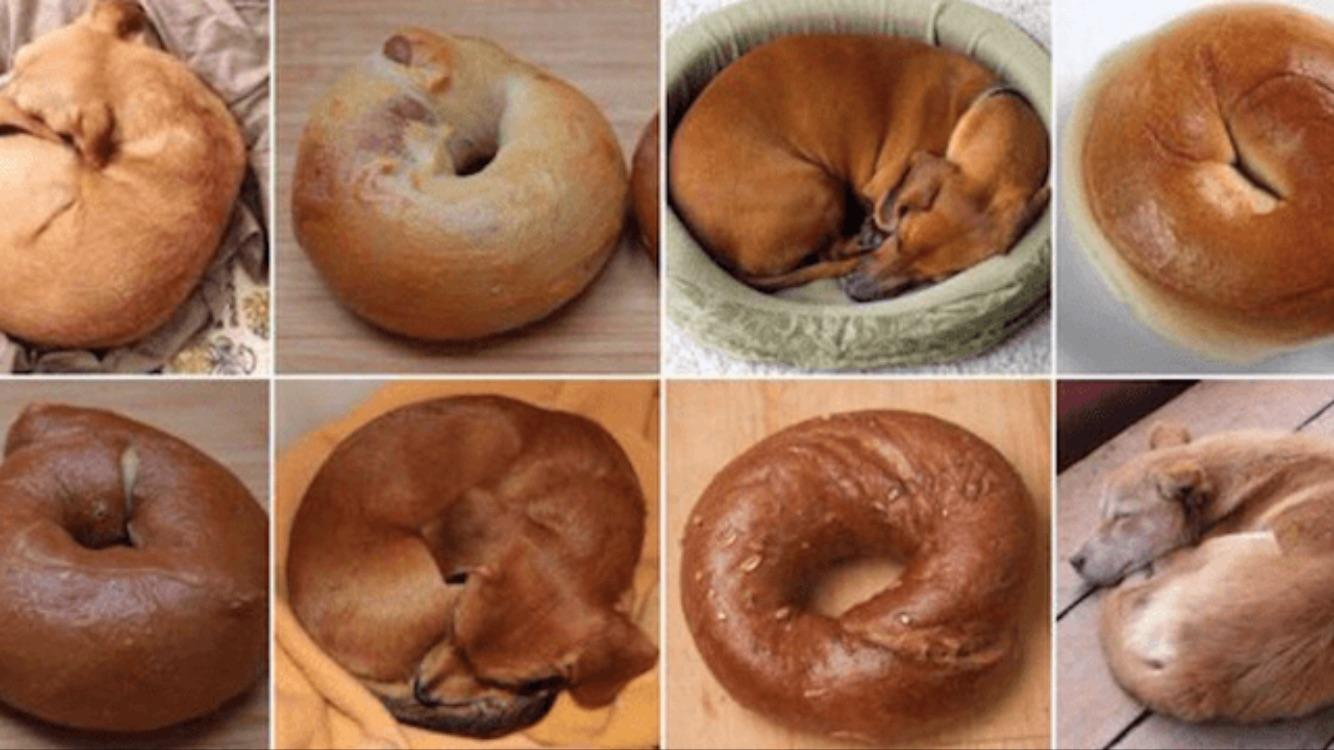
\includegraphics[width=15cm]{Bilder/dog_or_bagel.jpg}
		\caption{Hund oder Bagel?}
		\label{fig:dogBagel}
	\end{center}
\end{figure}

Es gibt Bilder, welche selbst für den Menschen schwer zu differenzieren sind (Beispiel Abbildung \ref{fig:dogBagel}). Ist nun ein Mensch nicht aufmerksam und sagt der Maschine das ein Bagel ein Hund ist, erlernt die Maschine falsche Bilder und sagt zukünftig auch Bagel als Hunde vorher. Aber auch durch richtiges Kennzeichnen der Bilder durch den Menschen, können solche Bilder zu Verzerrungen führen.
\\\\
Ein weiters Beispiel hierfür kommt aus der Autoindustrie. In Testreihen für autonomes Fahren stuften die Probanden (weil sie nicht aufmerksam waren) immer wieder das bestimmte Bild eines Menschen als Bild einer Tonne ein. Das System reagiert folgerichtig und wertet in einer kritischen Verkehrssituation das Überfahren einer (vermeintlichen) Tonne als verhältnismäßige Alternative, die möglichst wenig Schaden anrichtet \cite{trainingsDataKI}.

\section{Menschliche Fehler}
Den Faktor Mensch darf man bei der Bias Entstehung nicht vergessen. Konzeptionelle Fehler mangels an Wissen oder einem Missgeschick heraus fördern Fehlverhalten. Markante Defizite können ein funktionale KI-Entstehung komplett verhindern, sind in der Regel noch die besseren Missstände. Denn kleine Mängel, die nicht sofort auffallen, können in Produktion fatale Folgen haben.
\subsection{Falsche Zielsetzung}
Die Zielsetzung eines KNNs ist ein nicht zu unterschätzender Teil bei der KI Entwicklung. Setzt man hier den falschen Grundstein, können sich vermeidbare Fehlverhalten einer KI entwickelt.
\subsubsection{Falsche Ziel Definition}
Wenn man eine Aufgabe hat und diese Automatisieren möchte, greift man heute zutage gerne zur KI. KI ist modern und in aller Munde. Jedoch sollte einem im Klaren sein, dass künstliche Intelligenz kein Allheilmittel ist.
% ka
\subsubsection{Zu viele Ziele}
Viele Köche verderben den Brei. Diese Weisheit kann auch auf die Ziele von KNNs umgemünzt werden. Denn je mehr Ziele ein KNN hat, desto größer und komplexer muss ein KNN sein, um alle Fälle abdecken zu können. Je komplexer ein KNN ist, desto größer ist die Wahrscheinlichkeit, dass Fehler passieren. Auch ist sich das Netz deutlich unsicherer bei seinen Entscheidungen.
\\\\ % Ohne Quelle :(
Wenn man eine nahe zu perfekte KI mit einer Aufgabe erweitern möchte, hat das meist zu Folge, dass die KI nach der Erweiterung zwar mehr kann, jedoch seine ehemalige Hauptaufgabe nicht mehr so gut meistert wie zuvor.
% Beispiel: Baidu Gesichtserkennung (erkennt nur Asiaten)
\subsection{Falsche Modearchitektur Wahl}
Grundgedanke 'Je mehr Neuronen und Schichten eine Netz hat desto besser' ist falsch.
\subsection{Falsches Lernverhalten}
KI lernt einfachste Unterschiede
\\i.	Nicht Unterschied zwischen Auto und Boot sondern Untergrund(Wasser/Land)
\\ii.	Sehr Fehleranfällig z.B. Auto fährt durch flaches Wasser (KI -> Boot)
\chapter{Sicherheitsprobleme durch BIAS}

\section{Gefahren für Maschinen}
Google KI -> Kühlung von Maschinen
\section{Gefahren für Menschen}
Tesla Autopilot
\\Etc.
\section{Angriff auf KI}
Ist eine Künstliche Intelligenz sehr gut trainiert, erzielt sie in ihrem Aufgabebereich überragende Ergebnisse. Doch auch nahe zu perfekte KIs sind nicht unfehlbar. Durch methodisch gestaltete Störungen der Daten kann eine KI bewusst getäuscht werden und die Computer-Wahrnehmung in die Irre führen. Diese Art der Ausnutzung von KI Schwächen nennt man Adversarial Attacks, zu deutsch gegensätzlicher Angriff.
\subsubsection{Adversarial Attacks}
Bildererkennungssoftware ist besonders anfällig von dieser Art von Angriff. Hierbei legt man über das Bild bestimmte Pixelmuster, die für das menschliche Auge in der Regel im Gesamtbild untergehen. KIs hingegen registrieren jegliches Muster und nehmen sie in ihre Berechnungen mit auf. Als Ergebnis werden Bilder zum Teil massiv fehlinterpretiert. 
Im Folgenden Angriff wird mit einer Brille und dessen speziellen Muster, eine KI überlistet.
\label{section:BrilleAttack}
\begin{figure}[h]
	\begin{center}
		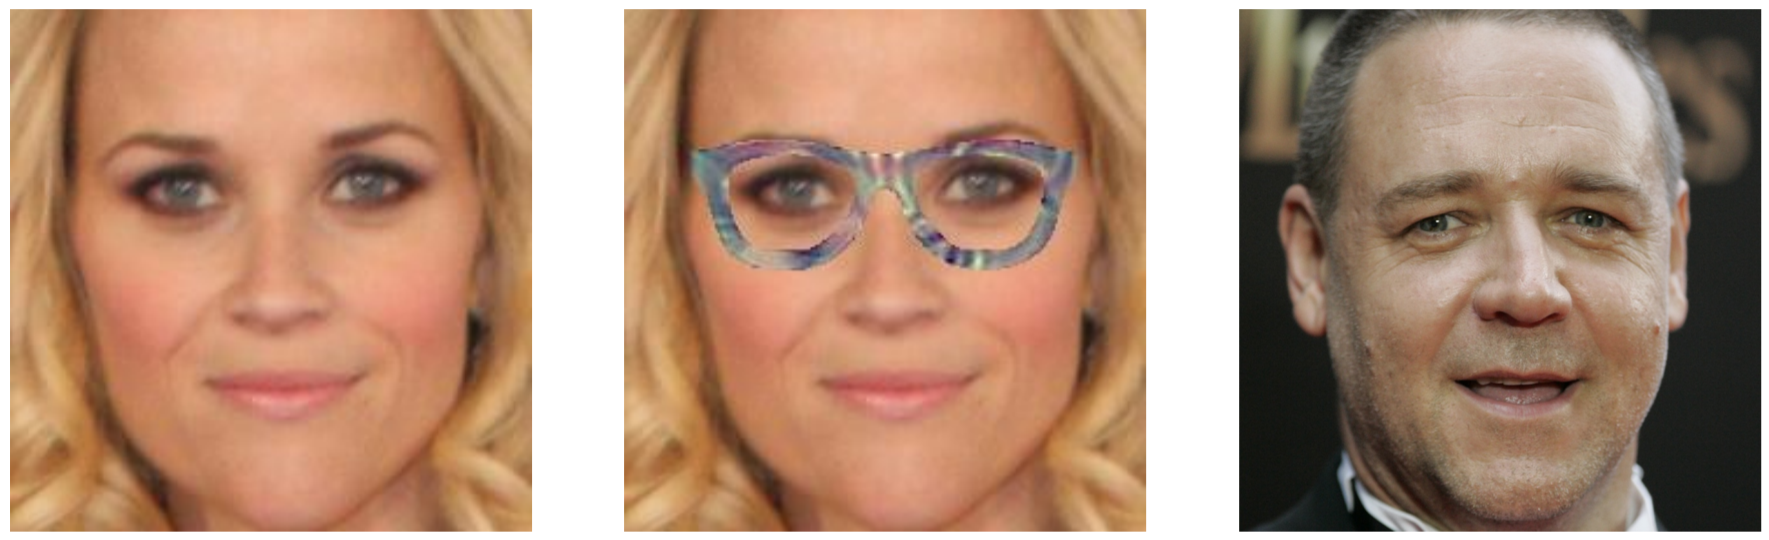
\includegraphics[width=15cm]{Bilder/Brille_Adversarial_Attack.png}
		\caption{Reese Witherspoon links korrekt identifiziert. Mitte Bild mit Adversarial Attack. Rechts Klassifizierung von Mitte als Russel Crowe}
		\label{fig:BrilleAttack}
	\end{center}
\end{figure}
% Paper https://www.cs.cmu.edu/~sbhagava/papers/face-rec-ccs16.pdf
Im linken Bild sieht man die amerikanische Schauspielerin Reese Witherspoon. Dieses Bild wird auch korrekt als sie selbst von der KI erkannt. Setzt man nun ihr eine spezielle Brille auf, beginnt das neuronale Netz Fehler zu begehen. Plötzlich erkennt die KI Reese Witherspoon mit Brille als Russel Crowe (Bild rechts).

%https://www.inovex.de/blog/machine-perception-face-recognition/
\chapter{Prävention}
\label{chapter:main}
\section{Passender Algorithmus zu Daten}

Im Abschnitt \ref{section:DataGarbage} wurden die Schwierigkeiten genannt, was passiert wenn ein Modell mit fehlerhaften Daten trainiert wurde und ab einem gewissen Grad es schwer wird diese fehlerhaften Vorhersagen zu verstehen und abzuändern.
\\\\
In der Annahme das nun dieses System richtig trainiert wurde, aber die zeitliche Komponente nicht beachtet, wie z.B. dass ein Panzer in Zukunft anders ausschauen könnte, kann es zu dem Problem kommen, das in Zukunft ein Panzer nicht mehr erkannt wird. Wie Stöcker 2019(\cite{stoecker}) bereits erwähnte, benötigt eine sich ändernde Gesellschaft auch kontinuierliche weiterlernende Algorithmen. 
\\\\
Solch ein Lernprozess wird auch als \textit{adaptive learning} bezeichnet, womit dem Effekt sich ändernder, d. h. dynamischer Datenumgebungen, concept drift bezeichnet, Rechnung getragen wird \cite{gama}. In DL-Algorithmen ist solche eine Umsetzung nicht trivial, aber das Beispiel von Sahoo et al. \cite{sahoo} zeigt auch die Machbarkeit auch in diesem Feld.
\\\\
Auch bei einem für Diskriminierung anfälligen Umfeld, wie im Beispiel von Abschnitt \ref{section:biasInTest}, muss besondere Sorgfalt bei der Wahl des passenden Algorithmus bedacht werden. Oftmals ist es unzureichend einzelne Attribute aus den Eingangsdaten auszuschließen, um beispielsweise eine algorithmische Diskriminierung bestimmter Personengruppen zu verhindern. Dies genügt jedoch in der Regel nicht, denn wie das Beispiel von Amazon zeigt, kann der Algorithmus Rückschlüsse anhand anderer Attribute ziehen(z.B. durch Frauenvereine).
\\\\
In diesem Kontext sollten System bevorzugt werden, welche in der Entwicklung solcher Algorithmen zusätzliche Einschränkungen einführen, um eine Diskriminierung aufgrund eines bestimmten Attributs, zu verhindern \cite{kamiran}.

\section{Nur ein Ziel}
\label{section:oneGoal}
Nimmt man das Beispiel aus dem Abschnitt \ref{section:OverUnderfitting} mit den Schränken und möchte der Maschine alle möglichen Schränke beibringen, kann dies wie in diesem Absatz bereits erläutert zu Overfitting führen. Das Ziel aus diesem Beispiel war zu komplex. Hier hätte man das Ziel einfacher halten und die Daten generalisieren sollen. Dass heißt sich auf Schränke beschränken die sofort als solche erkannt werden. Falls ein Schrank ein komplizierteres Aussehen hätte und durch den Algorithmus nicht erkannt worden wäre, wäre das besser als wenn der Algorithmus viele Autos als Schränke erkennt. 
\\\\
Solche Probleme treten häufig auf, da die Ziele meist zu komplex gehalten werden. Das führt zu einer großen Fehleranfälligkeit und somit zu Verzerrungen. Deswegen sollten die Ziele klar und einfach gehalten werden, um unnötige Komplexität zu vermeiden.

\section{Verfahren zum Validieren}
\label{section:validate}

Damit Vorurteile, Outliner oder falsche Bilder in den Daten nicht zu Problemen führen sollte diese zuvor überprüft werden. Beispiele dafür könnten folgende sein:
\begin{enumerate}
	\item Lektorat oder Peer-Review
	\item Das Vier-Augen-Prinzip (gegenseitige Kontrolle)
	\item Mehrheitsentscheide bei unterschiedlichen Ergebnissen
\end{enumerate}

Zudem sollte das Modell ausreichend validiert werden und die Performance gemessen werden. Denn wenn der Algorithmus z.B. bei der Diagnose von Krebs helfen soll, sollten die Ergebnisse nicht falsch sein.
\\\\
Würde man einen Datensatz in Trainings und Testdaten unterteilen, könnte es dazu kommen, das die Daten so perfekt aufgeteilt werden, dass er in dieser Aufteilung sehr gute Ergebnisse liefert. Falls nun aber ein Fall nur in den Testdaten vorhanden ist und somit nicht antrainiert wurde, jetzt aber in der realen Welt benötigt wurde, können die Ergebnisse trüben und das Modell könnte zu Problemen führen.
\\\\
Eine Möglichkeit um das zu verhindern, bietet die Cross Validierung. Anstelle eines extra Datensatzes, welcher zum Validieren der Daten genutzt wird, wird der Datensatz in viele kleine Blöcke unterteilt. In der Abbildung \ref{fig:crossValidierung} sind es 5. Danach werden 5 Durchläufe gemacht, in denen jeweils mit 4 unterschiedlichen aus diesen 5 Blöcken trainiert und mit einem davon getestet wird. Bei jedem Durchlauf entsteht ein Score, welche angibt, wie gut das Modell ist. Am Ende wird dann ein durchschnittlicher Score über diese 5 einzelnen gebildet, welcher die gesamt Performance des Modells angibt.

\begin{figure}[h]
	\begin{center}
		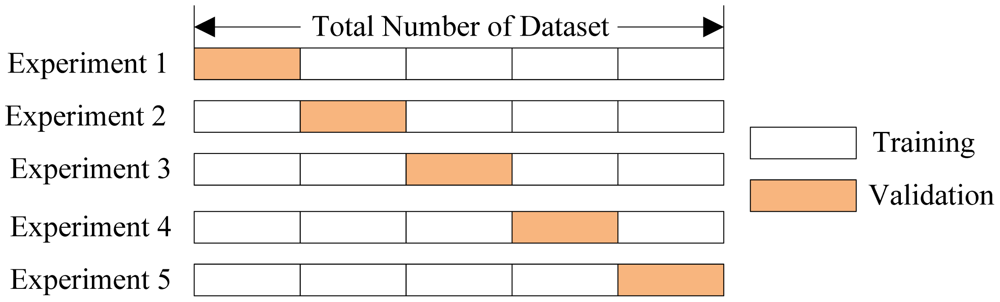
\includegraphics[width=15cm]{Bilder/crossValidierung.png}
		\caption{5 fache Cross Validierung}
		\label{fig:crossValidierung}
	\end{center}
\end{figure}

Mit diesem Score lässt sich das beste Modell ermitteln und man verhindert unbewusste Nebenwirkungen.

\section{Over- und Underfitting vermeiden}
\label{section:preventData}

Underfitting und Overfittung sind oft Fehler der Test-/Trainingsdaten Aufbereitung. Um Overfitting eventuell zu verhindern, kann ein einfacheres Ziel wie bereits in Absatz \ref{section:oneGoal} beschrieben, ausreichen. Dennoch gibt es Fälle wo das Ziel zu komplex ist oder zu wenig Daten vorhanden sind, um Underfitting oder Overfitting zu verhindern.

\subsection{Underfitting}

Anhand einer polynominialen Regression kann man verdeutlichen, wie Underfitting vermieden werden könnte. Um dies zu erreichen, muss der erwartete Wert einer Variable als Polynom n-ten Grades modelliert werden, welches dann wiederum das allgemeine Polynom ergibt. Wenn wir den Grad ${n}$ des Polynoms erhöhen, nimmt der Trainingsfehler generell ab. Die allgemeine Gleichung eines Polynoms ist folgende:

${\displaystyle y=\beta_{0}+\beta_{1}x+\beta_{2}x^{2}+...+\beta_{n}^n+\epsilon}$

Aber hier muss aufgepasst werden. Denn wie in der Abbildung \ref{fig:polyReg} zu sehen sinkt zur gleichen Zeit der Cross Validierungsfehler solange wir n bis zu einem gewissen Punkt erhöhen, nach diesem Punkt steigt der Fehler und Overfitting wird das Problem.

\begin{figure}[h]
	\begin{center}
		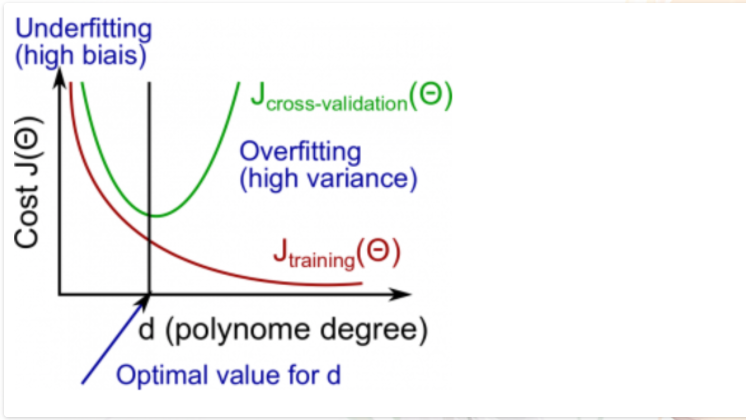
\includegraphics[width=15cm]{Bilder/polynomeRegression.png}
		\caption{Polynominale Regression}
		\label{fig:polyReg}
	\end{center}
\end{figure}

\subsection{Overfitting}

Eine Möglichkeit um Overfitting zu vermeiden bietet die bereits in Abschnitt \ref{section:validate} Cross Validierung. Eine andere kann durch das erhöhen der Flexibilität des Models erreicht werden. Dabei sollte dies aber in Grenzen bleiben, da ansonsten das gleiche wie bei Underfitting passiert. Um die Flexibilität zu erhöhen können Regulierungstechniken benutzt werden.
\\\\
Durch die Regularisierung wird wenn die Komplexität eines Models zunimmt, eine Strafe angehängt. Der Regularisierungsparameter (${\lambda}$) bestraft alle Parameter mit Ausnahme des markierten Bereichs in Abbildung \ref{fig:regFunc}, sodass das Modell die Daten verallgemeinert und nicht überanpasst.

\begin{figure}[h]
	\begin{center}
		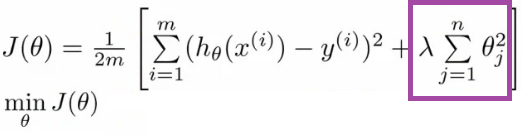
\includegraphics[width=10cm]{Bilder/regFunc.png}
		\caption{Regularisierung in Loss Funktion}
		\label{fig:regFunc}
	\end{center}
\end{figure}

Wenn in der Abbildung \ref{fig:regFunc} die Komplexität steigt, wird durch die Regulierung eine Strafe für höhere Terme hinzugefügt. Dass hat zur Folge, dass die Wichtigkeit solcher langen Terme sinkt und zugleich die Komplexität des Models weniger wird.
\\\\
Beispiele für solche Techniken sind folgende:

\begin{enumerate}
	\item L1 Regulierung (Lasso Regulierung)
	\item L2 Regulierung (Ridge Regulierung)
	\item Elastic net
\end{enumerate}


\chapter{Fazit}
Thema ist größer als hier beschreibbar
\\Evtl. Deep Fake
http://iphome.hhi.de/samek/pdf/LapNCOMM19.pdf
https://ujjwalkarn.me/2016/08/11/intuitive-explanation-convnets/



\backmatter
%%%%%%%%%%%%%%%%%%%
%% create tables list
%%%%%%%%%%%%%%%%%%%
%\listoftables

%%%%%%%%%%%%%%%%%%%
%% create listings list
%%%%%%%%%%%%%%%%%%%
%\lstlistoflistings
%\addcontentsline{toc}{chapter}{Listings}

\cleardoublepage
\phantomsection
\addcontentsline{toc}{chapter}{Literatur}
\printbibliography

\end{document}
